\chapter{A constant with many exact faces}
\label{ch:constant}

Catalan's constant begins with an unusually accessible definition. Its terms are rational, their signs alternate, and its value can be enclosed without assuming anything about irrationality. The difficulty appears when one asks what kind of number the limit is. A definition, an integral, a recurrence and a long decimal expansion each give access to the same number. None of these descriptions alone supplies the arithmetic conclusion.

This chapter fixes the analytic object before we introduce rational approximants. All integral identities and interval bounds below are proved directly. The finite computations in the accompanying bundle use these bounds to decide signs. They do not use a floating point approximation to make an exact decision.

\section{Definition and the question being asked}

\begin{definition}[Catalan's constant]
\label{def:c01-G}
The real number studied in this book is
\begin{equation}
G=\sum_{k=0}^{\infty}\frac{(-1)^k}{(2k+1)^2}.
\label{eq:c01-definition}
\end{equation}
The series converges absolutely because
\[
\sum_{k=0}^{\infty}\frac1{(2k+1)^2}
\leq\sum_{j=1}^{\infty}\frac1{j^2}<\infty.
\]
\end{definition}

The familiar decimal display begins
\[
G\approx0.91596559417721901505460351493238411077.
\]
The approximation sign matters. A decimal is a coordinate for seeing the number, while a rational enclosure is evidence for a particular numerical assertion. A proof of irrationality requires a different assertion again.

\begin{conjecture}[The irrationality question]
\label{conj:c01-irrationality}
Catalan's constant does not belong to $\Q$.
\end{conjecture}

The checked material for this edition does not establish this conjecture. The literature record includes a September 2026 preprint claiming a proof and a subsequent primary note identifying an incomplete asymptotic derivation \cite{Sun2026,Wachs2026}. The later chapters state that record with its date and scope. The constructions developed here do not depend on accepting the claimed proof.

Irrationality would mean that no integers $a,b$ with $b\ne0$ satisfy $G=a/b$. Transcendence would mean that no nonzero polynomial with integer coefficients vanishes at $G$. These are different questions. The second implies the first, because a rational number $a/b$ is a zero of the polynomial $bx-a$. Our target throughout is the first assertion.

\begin{figure}[tbp]
\centering
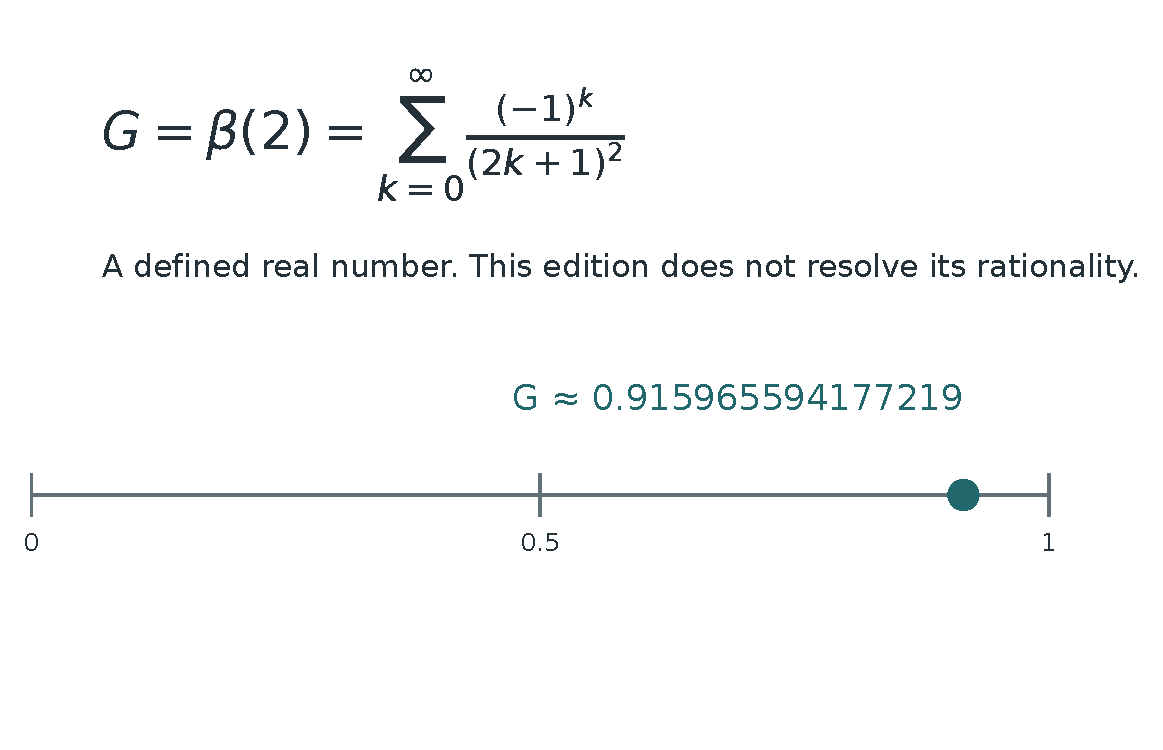
\includegraphics[width=0.94\linewidth]{../visual/figures/01_constant.pdf}
\caption{The same constant appears through a convergent series and through exact integral representations. The displayed decimal supplies orientation. The formulas, rather than the printed digits, define the object.}
\label{fig:c01-constant}
\end{figure}

\subsection{The Dirichlet beta family}

For real $s>1$, the Dirichlet beta value is
\begin{equation}
\beta(s)=\sum_{k=0}^{\infty}\frac{(-1)^k}{(2k+1)^s}.
\label{eq:c01-beta}
\end{equation}
Absolute convergence follows from comparison with $\sum j^{-s}$. Thus $G=\beta(2)$. The alternating series also defines $\beta(s)$ for $s>0$, though absolute convergence is no longer available throughout that wider range. At $s=1$, integration of the finite geometric expansion of $(1+x^2)^{-1}$ gives $\beta(1)=\pi/4$. The integrated remainder is bounded by $\int_0^1x^{2N}\dd x=(2N+1)^{-1}$ and tends to zero, so this passage does not require absolute convergence of the beta series at $1$.

The family gives useful context without collapsing its separate arithmetic questions. Zudilin proved that at least one of
\[
\beta(2),\ \beta(4),\ \beta(6),\ \beta(8),\ \beta(10),\ \beta(12)
\]
is irrational \cite{Zudilin2019}. This is a disjunction. It permits the irrational member to be a value other than $\beta(2)$. A proof about the collection therefore cannot be inserted as a proof about $G$. The precise source contract is LC09 in the evidence bundle.

\section{Alternating partial sums give rational intervals}

Write
\begin{equation}
s_N=\sum_{k=0}^{N-1}\frac{(-1)^k}{(2k+1)^2},\qquad N\geq0,
\label{eq:c01-partial-sum}
\end{equation}
where $s_0=0$ is the empty sum. Thus $N$ counts retained terms, as it does in the visual guide. Each $s_N$ is an exact rational number. The terms decrease strictly in magnitude to zero. Grouping successive terms shows that the even partial sums increase and the odd partial sums decrease. These two sequences approach the same limit.

\begin{proposition}[Alternating enclosure]
\label{prop:c01-alternating}
For every integer $r\geq0$,
\begin{equation}
s_{2r}<G<s_{2r+1}.
\label{eq:c01-parity-enclosure}
\end{equation}
For every integer $N\geq0$,
\begin{equation}
0<(-1)^N(G-s_N)<\frac1{(2N+1)^2}.
\label{eq:c01-alternating-error}
\end{equation}
\end{proposition}

\begin{proof}
The difference between two consecutive even sums is
\[
s_{2r+2}-s_{2r}
=\frac1{(4r+1)^2}-\frac1{(4r+3)^2}>0.
\]
Similarly,
\[
s_{2r+3}-s_{2r+1}
=-\frac1{(4r+3)^2}+\frac1{(4r+5)^2}<0.
\]
Consecutive sums differ by a term tending to zero, so the increasing even sums and decreasing odd sums have the same limit $G$. Strictness follows because the next sum of the same parity lies strictly between the current endpoint and the limit on the other side.

To obtain the error bound, apply this enclosure to $s_N$ and $s_{N+1}$. The limit lies strictly between them. Their distance is $(2N+1)^{-2}$, and the direction from $s_N$ to $s_{N+1}$ has sign $(-1)^N$.
\end{proof}

For example,
\[
s_0=0,\qquad s_1=1,\qquad s_2=\frac89,\qquad
s_3=\frac{209}{225},\qquad
s_4=\frac{10016}{11025}.
\]
Hence
\begin{equation}
\frac{10016}{11025}<G<\frac{209}{225}.
\label{eq:c01-small-bracket}
\end{equation}
These statements use only rational arithmetic. The strict inequality also proves $0<G<1$, which will simplify later tail estimates.

\begin{figure}[tbp]
\centering
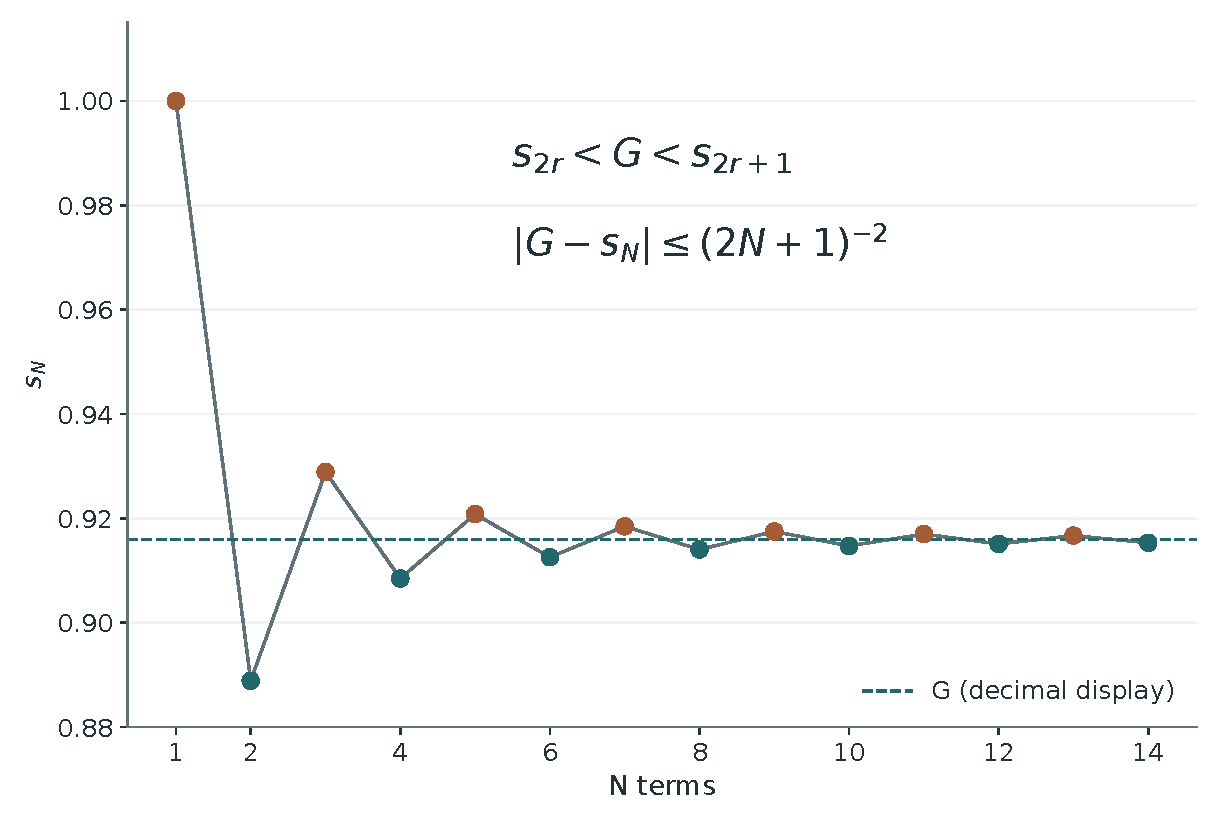
\includegraphics[width=0.94\linewidth]{../visual/figures/02_alternating_series.pdf}
\caption{Even and odd partial sums approach the common limit from opposite sides. Their errors are controlled by the next omitted term. Every partial sum represented in the figure is rational.}
\label{fig:c01-alternating}
\end{figure}

The error bound is transparent, but its decay is slow. To make the next omitted term smaller than $10^{-d}$, one needs $2N+1>10^{d/2}$. Increasing numerical accuracy this way rapidly becomes expensive. The Euler transform below produces a much faster certified enclosure. Before using it, we establish the positive integral that controls its terms.

\section{Three exact integral descriptions}

\subsection{A logarithmic integral}

\begin{lemma}[A basic moment]
\label{lem:c01-moment}
For every real $a>-1$,
\begin{equation}
\int_0^1x^a(-\log x)\,\dd x=\frac1{(a+1)^2}.
\label{eq:c01-moment}
\end{equation}
The integral is understood as an improper integral at $0$.
\end{lemma}

\begin{proof}
Set $x=e^{-t}$. Then $-\log x=t$, $\dd x=-e^{-t}\dd t$, and the integral becomes
\[
\int_0^{\infty}t e^{-(a+1)t}\,\dd t.
\]
Integration by parts gives $(a+1)^{-2}$. The boundary term at infinity is zero because an exponential with positive decay rate dominates $t$. The boundary term at zero is also zero.
\end{proof}

\begin{proposition}[Single integral]
\label{prop:c01-log-integral}
Catalan's constant satisfies
\begin{equation}
G=\int_0^1\frac{-\log x}{1+x^2}\,\dd x.
\label{eq:c01-log-integral}
\end{equation}
\end{proposition}

\begin{proof}
For $0\leq x<1$, the geometric expansion is
\[
\frac1{1+x^2}=\sum_{k=0}^{\infty}(-1)^kx^{2k}.
\]
The integrated absolute values of the proposed terms have finite sum:
\[
\sum_{k=0}^{\infty}\int_0^1x^{2k}(-\log x)\,\dd x
=\sum_{k=0}^{\infty}\frac1{(2k+1)^2}<\infty.
\]
Therefore the series of integrable functions can be summed under the integral. The moment identity gives the defining series for $G$. The point $x=1$ has measure zero and does not affect the integral.
\end{proof}

The singularity in $-\log x$ is integrable. This is a useful example of why an unbounded integrand is not the same as an infinite integral. In fact, $\int_0^1-\log x\,\dd x=1$. The factor $(1+x^2)^{-1}$ is bounded between $1/2$ and $1$, so the integral representation independently places $G$ between $1/2$ and $1$.

\subsection{An arctangent and a logarithmic tangent}

\begin{proposition}[Arctangent and tangent forms]
\label{prop:c01-tangent}
The following equalities hold:
\begin{equation}
G=\int_0^1\frac{\arctan x}{x}\,\dd x
=-\int_0^{\pi/4}\log(\tan\theta)\,\dd\theta.
\label{eq:c01-tangent-forms}
\end{equation}
The integrand $\arctan x/x$ is assigned its continuous value $1$ at $x=0$.
\end{proposition}

\begin{proof}
For $0<\delta<1$, integration by parts gives
\[
\int_\delta^1\frac{\arctan x}{x}\,\dd x
=-\arctan(\delta)\log\delta
-\int_\delta^1\frac{\log x}{1+x^2}\,\dd x.
\]
The boundary expression tends to zero as $\delta\downarrow0$, since $0\leq\arctan\delta\leq\delta$ and $\delta\abs{\log\delta}\to0$. The first equality follows from Proposition~\ref{prop:c01-log-integral}.

For the second equality, substitute $x=\tan\theta$ into the logarithmic integral. On $0<\theta\leq\pi/4$,
\[
\frac{\dd x}{1+x^2}=\dd\theta.
\]
The substitution is valid first on a truncated interval. Its limit exists by the integrability already established for $-\log x$.
\end{proof}

The logarithmic tangent form will later identify an integral normalization at index zero. That check is especially valuable because a constant factor in a linear form changes its normalization even when its qualitative decay is unaffected. We will use the equality just proved, rather than assume the normalization from a printed formula.

\subsection{A double integral over a square}

\begin{proposition}[Elementary double integral]
\label{prop:c01-double}
Catalan's constant also satisfies
\begin{equation}
G=\int_0^1\int_0^1\frac{\dd x\,\dd y}{1+x^2y^2}.
\label{eq:c01-double}
\end{equation}
\end{proposition}

\begin{proof}
One proof integrates with respect to $y$. For $x>0$,
\[
\int_0^1\frac{\dd y}{1+x^2y^2}=\frac{\arctan x}{x}.
\]
The value at $x=0$ is $1$. Proposition~\ref{prop:c01-tangent} now gives the result.

There is also a direct series justification. Expanding $(1+x^2y^2)^{-1}$ on the square except at the corner $(1,1)$ gives geometric terms $(-1)^kx^{2k}y^{2k}$. Their integrated absolute values sum to
\[
\sum_{k=0}^{\infty}\left(\int_0^1x^{2k}\,\dd x\right)^2
=\sum_{k=0}^{\infty}\frac1{(2k+1)^2}<\infty.
\]
Thus summation and integration may be interchanged, giving the defining series again.
\end{proof}

The double integral is bounded and positive on a compact square. The logarithmic integral has an integrable endpoint singularity. Both represent exactly the same number. Their different analytic forms permit different transformations, but their arithmetic classification remains a separate obligation.

\section{An Euler transform with an exact tail bound}

Let
\[
a_k=\frac1{(2k+1)^2},\qquad k\geq0,
\]
and define the positive difference convention
\begin{equation}
\Delta a_k=a_k-a_{k+1}.
\label{eq:c01-difference-convention}
\end{equation}
The sign convention is fixed here because the other common convention would change every odd difference. Iteration gives
\begin{equation}
\Delta^j a_0=\sum_{k=0}^{j}(-1)^k\binom jk\frac1{(2k+1)^2}.
\label{eq:c01-finite-difference}
\end{equation}
This is an exact rational number for every $j$.

\begin{lemma}[Positive differences]
\label{lem:c01-positive-differences}
For every integer $j\geq0$,
\begin{equation}
\Delta^j a_0
=\int_0^1(1-x^2)^j(-\log x)\,\dd x,
\qquad 0<\Delta^j a_0\leq1.
\label{eq:c01-positive-differences}
\end{equation}
\end{lemma}

\begin{proof}
Insert the moment formula into the finite sum in \eqref{eq:c01-finite-difference}. A finite sum can be interchanged with an integral without any convergence issue. The binomial theorem gives
\[
\sum_{k=0}^{j}(-1)^k\binom jkx^{2k}=(1-x^2)^j.
\]
The integrand is positive for $0<x<1$. It is at most $-\log x$, whose integral is $1$.
\end{proof}

\begin{theorem}[Certified Euler enclosure]
\label{thm:c01-euler}
Define
\begin{equation}
E_N=\sum_{j=0}^{N}\frac{\Delta^j a_0}{2^{j+1}},\qquad N\geq0.
\label{eq:c01-E}
\end{equation}
Then
\begin{equation}
G=\sum_{j=0}^{\infty}\frac{\Delta^j a_0}{2^{j+1}},
\qquad
E_N<G<E_N+2^{-N-1}.
\label{eq:c01-euler-enclosure}
\end{equation}
More precisely,
\begin{equation}
G-E_N
=\int_0^1\frac{-\log x}{1+x^2}
\left(\frac{1-x^2}{2}\right)^{N+1}\,\dd x.
\label{eq:c01-euler-remainder}
\end{equation}
\end{theorem}

\begin{proof}
By the preceding lemma all terms of the series are nonnegative. Monotone convergence permits the sum to pass under the integral. For $0\leq x\leq1$,
\[
\sum_{j=0}^{\infty}\frac{(1-x^2)^j}{2^{j+1}}
=\frac1{1+x^2}.
\]
The resulting integral is $G$ by Proposition~\ref{prop:c01-log-integral}.

The finite geometric identity is
\[
\sum_{j=0}^{N}\frac{(1-x^2)^j}{2^{j+1}}
=\frac{1-((1-x^2)/2)^{N+1}}{1+x^2}.
\]
Integration gives the exact remainder formula. Its integrand is positive on $(0,1)$, so $G-E_N>0$. Since $(1-x^2)/2\leq1/2$,
\[
G-E_N\leq2^{-N-1}G<2^{-N-1}.
\]
This gives the stated enclosure. An alternative bound sums the omitted terms using $\Delta^ja_0\leq1$, with the same geometric tail $2^{-N-1}$.
\end{proof}

The stronger intermediate inequality also gives
\begin{equation}
G\leq\frac{E_N}{1-2^{-N-1}}.
\label{eq:c01-euler-sharper}
\end{equation}
The denominator is positive for every $N\geq0$. The release computations use the simpler interval $[E_N,E_N+2^{-N-1}]$, because that interval has an immediate rational width and is already sufficient for the tested signs.

\begin{example}[Small Euler intervals]
The first difference values are
\[
\Delta^0a_0=1,\qquad \Delta a_0=\frac89,\qquad
\Delta^2a_0=\frac{184}{225}.
\]
They give
\[
E_0=\frac12,\qquad E_1=\frac{13}{18},\qquad
E_2=\frac{371}{450}.
\]
Thus, for example,
\[
\frac{371}{450}<G<\frac{1709}{1800}.
\]
These short transformed sums are useful for checking conventions. Their principal advantage appears as $N$ grows, because the certified width decreases geometrically.
\end{example}

The independent audit retains $j=0,\ldots,1000$. Its exact rational endpoints differ by $2^{-1001}$. The finite differences and endpoint numerators are recorded in the evidence bundle. The preceding theorem proves the tail bound for every $N$. The program computes the finite rational portion at one chosen $N$ and checks its internal arithmetic. These are complementary forms of evidence with different scopes.

\section{What a certified interval can decide}

Suppose $l\leq G\leq h$ is a proven rational enclosure, and suppose $a,b\in\Q$. Then the interval for $aG-b$ is
\begin{equation}
\begin{cases}
[al-b,ah-b],&a\geq0,\\
[ah-b,al-b],&a<0.
\end{cases}
\label{eq:c01-linear-interval}
\end{equation}
All endpoints are rational. If the entire interval is positive, the form is positive. If the entire interval is negative, the form is negative. If it contains zero, the enclosure has not decided the sign. That last outcome is a limitation of the chosen certificate, not evidence that the form actually vanishes.

This procedure makes the finite sign checks reproducible. It also limits their interpretation. A finite family of certified nonzero forms proves nonvanishing for those forms. It does not prove a universal assertion about all indices. A long decimal expansion cannot replace the rational enclosure when a coefficient is large enough to amplify the final rounding error.

The next chapter explains why even an infinite family of nonzero real errors is not enough. Their coefficients must become integers, and the errors after that arithmetic operation must still tend to zero.

\chapter{The arithmetic threshold for irrationality}
\label{ch:lattice}

The real approximation problem asks for rational numbers near $G$. The arithmetic problem asks for nonzero integer linear forms in $G$ whose absolute values tend to zero. These problems are related, but the passage between them has a cost. A coefficient denominator can absorb the analytic gain. A common divisor can recover some of that gain. Nonvanishing has to survive the whole construction.

The threshold is elementary enough to prove in a few lines. Its applications are demanding because all its hypotheses must hold together. This chapter states the criterion precisely, gives rational counterexamples to weaker assertions, and sets up the rate accounting used for the later filters.

\section{Rational numbers leave a fixed gap}

\begin{lemma}[Rational lattice gap]
\label{lem:c02-gap}
Suppose $\alpha=a/b$ with $a\in\Z$ and $b\in\Z_{>0}$. For every pair $P,Q\in\Z$, either $Q\alpha-P=0$ or
\begin{equation}
\abs{Q\alpha-P}\geq\frac1b.
\label{eq:c02-gap}
\end{equation}
\end{lemma}

\begin{proof}
Multiplication by $b$ gives
\[
b(Q\alpha-P)=Qa-Pb\in\Z.
\]
A nonzero integer has absolute value at least $1$. Division by the positive integer $b$ gives the result. No coprimality hypothesis is needed.
\end{proof}

For a fixed rational $\alpha$, every integer form $Q\alpha-P$ lies in the discrete set $b^{-1}\Z$. Its nonzero values cannot enter the open interval $(-1/b,1/b)$. The denominator $b$ need not be known to use this obstruction. If a constructed infinite family has nonzero values tending to zero, it eventually violates the gap for any proposed $b$.

\begin{theorem}[Integer form criterion]
\label{thm:c02-criterion}
Let $\alpha\in\R$. Suppose there are integer pairs $(P_j,Q_j)$ for $j\geq1$ such that
\begin{equation}
0<\abs{Q_j\alpha-P_j}\longrightarrow0.
\label{eq:c02-form-criterion}
\end{equation}
Then $\alpha$ is irrational. The same conclusion holds if these conditions are verified along any infinite subsequence.
\end{theorem}

\begin{proof}
If $\alpha=a/b$ were rational with $b>0$, Lemma~\ref{lem:c02-gap} would bound every nonzero form below by $1/b$. This contradicts convergence to zero. Restricting to a subsequence does not change the argument.
\end{proof}

\begin{figure}[tbp]
\centering
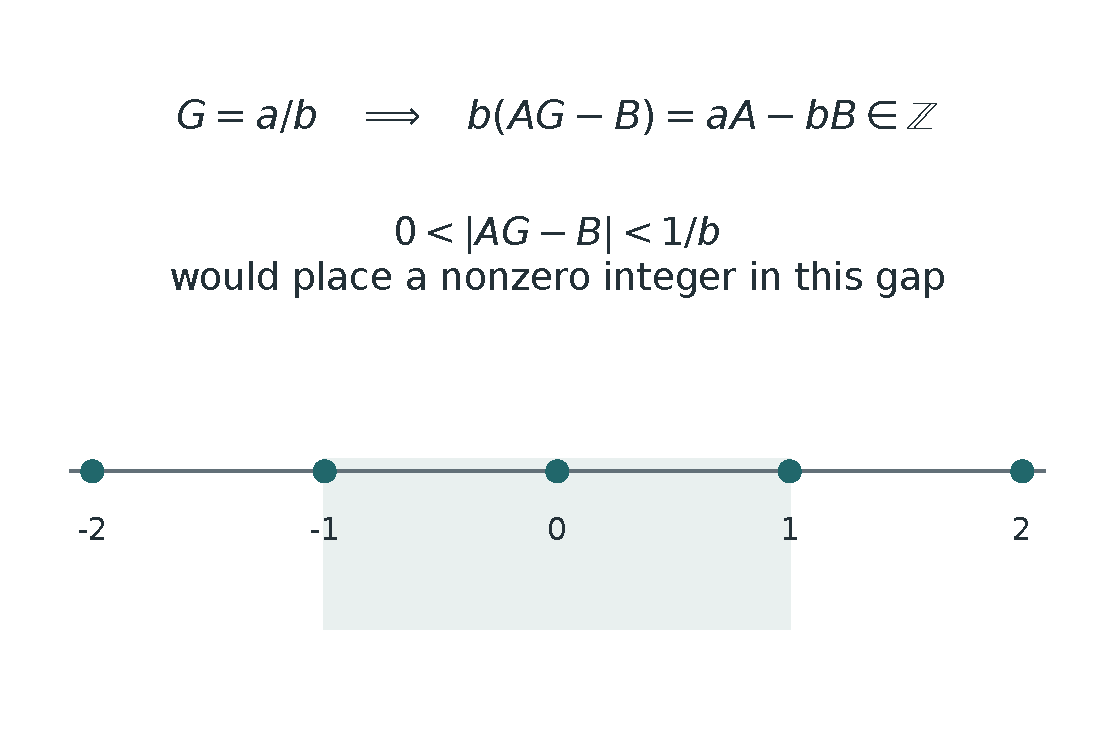
\includegraphics[width=0.94\linewidth]{../visual/figures/06_rationality_lattice.pdf}
\caption{Under the assumption $G=a/b$, integer linear forms lie on a lattice with spacing $1/b$. A sequence of nonzero forms approaching zero would contradict that spacing. The spacing is conceptual here because the hypothetical denominator is unknown.}
\label{fig:c02-lattice}
\end{figure}

The theorem separates three obligations. The coefficients must be integers. The forms must be nonzero at the indices being used. Their absolute values must approach zero. It is possible to establish any two while the third remains open.

For instance, setting $P_j=Q_j=0$ gives integer coefficients and zero error at every index, but proves nothing. Taking a rational approximation with a tiny error gives a small real form, but its coefficients may have large rational denominators. Clearing those denominators may keep the resulting integer form far from zero. These examples explain why the hypotheses are kept distinct throughout this book.

\subsection{Why the criterion is also a characterization}

The criterion is sufficient for irrationality. Conversely, every irrational real number admits such a family. This observation clarifies the role of the later constructions. The existence of small integer forms is not itself a novel definition of irrationality. The research problem is to construct and justify them for a specific constant.

\begin{proposition}[Elementary approximation by integer forms]
\label{prop:c02-pigeonhole}
If $\alpha$ is irrational, then for every integer $H\geq1$ there are integers $P,Q$ with $1\leq Q\leq H$ satisfying
\begin{equation}
0<\abs{Q\alpha-P}<\frac1H.
\label{eq:c02-pigeonhole}
\end{equation}
In particular, an infinite family as in Theorem~\ref{thm:c02-criterion} exists.
\end{proposition}

\begin{proof}
Consider the $H+1$ fractional parts of $0,\alpha,2\alpha,\ldots,H\alpha$. Partition $[0,1)$ into $H$ intervals of length $1/H$, using half open intervals. Two fractional parts lie in one interval. Their difference has absolute value strictly smaller than $1/H$. Subtracting the corresponding multiples of $\alpha$ gives $Q\alpha-P$ with $1\leq Q\leq H$ after choosing the order of the two indices.

The form is nonzero because $\alpha$ is irrational and $Q\ne0$. Choosing such a pair for every $H$ gives nonzero forms tending to zero. The denominators $Q$ cannot remain bounded. For any fixed finite set of positive $Q$, the distances from $Q\alpha$ to the nearest integers have a positive minimum. That minimum would contradict the bound as $H\to\infty$.
\end{proof}

This proof assumes irrationality in order to ensure nonvanishing. It cannot be used to prove irrationality of $G$ by inserting $\alpha=G$ before that fact is known. The lattice criterion runs in the other direction: first establish small nonzero forms by independent mathematics, then deduce irrationality.

\section{Approximation error and denominator are coupled}

Let $P_j/Q_j$ be rational approximants written in lowest terms, with $Q_j>0$. Their ordinary errors and their integer form errors are related by
\begin{equation}
\abs{Q_j\alpha-P_j}
=Q_j\abs{\alpha-\frac{P_j}{Q_j}}.
\label{eq:c02-error-conversion}
\end{equation}
Thus a plot of the ordinary error omits one factor from the arithmetic test. A rapid decrease in that plot can coexist with a denominator that grows just as rapidly.

\begin{corollary}[Reduced rational approximation criterion]
\label{cor:c02-reduced}
Suppose $P_j/Q_j$ is in lowest terms, $Q_j>0$, and $P_j/Q_j\ne\alpha$ at all indices used. If
\begin{equation}
Q_j\abs{\alpha-\frac{P_j}{Q_j}}\longrightarrow0,
\label{eq:c02-reduced-condition}
\end{equation}
then $\alpha$ is irrational.
\end{corollary}

\begin{proof}
The left side equals the absolute value of the nonzero integer form $Q_j\alpha-P_j$. Apply Theorem~\ref{thm:c02-criterion}.
\end{proof}

Reduction to lowest terms is not necessary for the theorem, but it gives the smallest denominator belonging to that rational number. If a common factor is left in $P_j,Q_j$, the form is multiplied by that factor. Keeping a redundant factor can conceal an available decay margin. Removing it cannot create nonvanishing if the original form was zero.

\begin{proposition}[Separation from a rational target]
\label{prop:c02-rational-distance}
If $\alpha=a/b$ with $b>0$ and $P/Q\ne\alpha$ with $P\in\Z$, $Q\in\Z_{>0}$, then
\begin{equation}
\abs{\alpha-\frac PQ}\geq\frac1{bQ}.
\label{eq:c02-rational-distance}
\end{equation}
\end{proposition}

\begin{proof}
The numerator of the difference is the nonzero integer $aQ-bP$:
\[
\abs{\frac ab-\frac PQ}=\frac{\abs{aQ-bP}}{bQ}\geq\frac1{bQ}.
\]
\end{proof}

This lower bound explains a familiar sufficient exponent. If distinct approximants have $Q_j\to\infty$ and
\begin{equation}
\abs{\alpha-\frac{P_j}{Q_j}}\leq C Q_j^{-\theta}
\label{eq:c02-exponent-bound}
\end{equation}
for a fixed constant $C>0$ and an exponent $\theta>1$, then multiplying by $Q_j$ gives a quantity tending to zero. The criterion applies. An upper bound with $\theta\leq1$ does not supply that conclusion on its own. It may still describe useful approximation, and another argument may still prove irrationality, but this particular inequality does not cross the required threshold.

\subsection{Two rational counterexamples}

\begin{example}[A convergent rational sequence with a fixed form error]
\label{ex:c02-linear-rational}
Let $\alpha=1/2$ and take
\[
\frac{P_n}{Q_n}=\frac{n}{2n+1},\qquad n\geq1.
\]
The numerator and denominator are coprime because any common divisor of $n$ and $2n+1$ divides $1$. The ordinary error is
\[
\frac12-\frac{n}{2n+1}=\frac1{2(2n+1)}\longrightarrow0.
\]
Nevertheless,
\[
Q_n\alpha-P_n=\frac12
\]
for every $n$. The approximants are distinct from the target, all coefficients are integers, and the approximations converge. The integer form does not tend to zero.
\end{example}

\begin{example}[Exponential approximation to a rational number]
\label{ex:c02-exponential-rational}
Again let $\alpha=1/2$. For $n\geq2$, set
\[
Q_n=2^n,\qquad P_n=2^{n-1}+1.
\]
The numerator is odd, so $P_n/Q_n$ is reduced. We have
\begin{equation}
\frac{P_n}{Q_n}=\frac12+2^{-n},\qquad
\abs{\alpha-\frac{P_n}{Q_n}}=2^{-n}.
\label{eq:c02-exponential-rational}
\end{equation}
The real error decreases exponentially. Yet
\[
Q_n\alpha-P_n=-1
\]
at every index. Exponential convergence of the ordinary error is therefore insufficient without the denominator comparison.
\end{example}

The second example can also be written as a failure of denominator clearing. The rational coefficient form
\[
\ell_n=\alpha-\left(\frac12+2^{-n}\right)=-2^{-n}
\]
is nonzero and tends to zero. Its second coefficient is not an integer. Multiplication by $2^n$ makes both coefficients integral and gives the constant form $-1$. The analytic gain has been exactly consumed by the arithmetic scale.

These counterexamples are deliberately elementary. They prevent a seductive but invalid inference: a known recurrence producing rapidly convergent rational approximants cannot settle irrationality until the actual coefficient denominators have been controlled.

\section{Clearing rational coefficients}

In the later chapters the starting form is
\begin{equation}
\ell_j=u_j\alpha-v_j,\qquad u_j,v_j\in\Q.
\label{eq:c02-rational-form}
\end{equation}
Choose a positive integer $D_j$ for which $D_ju_j$ and $D_jv_j$ are integers. Then
\begin{equation}
L_j=D_j\ell_j=(D_ju_j)\alpha-D_jv_j
\label{eq:c02-cleared-form}
\end{equation}
has integer coefficients. Its size is $D_j\abs{\ell_j}$, so the clearance factor must be included in any decay estimate.

Such a $D_j$ always exists for one finite rational pair. Write $u_j=a_j/b_j$ and $v_j=c_j/d_j$ in lowest terms with positive denominators. The smallest positive common clearing factor is
\begin{equation}
D_j^{\min}=\operatorname{lcm}(b_j,d_j).
\label{eq:c02-minimal-clearance}
\end{equation}
Indeed, integrality of $D_ja_j/b_j$ forces $b_j\mid D_j$ by coprimality, and integrality of $D_jc_j/d_j$ forces $d_j\mid D_j$. Conversely, their least common multiple clears both denominators.

A theorem may provide a larger convenient scale than the minimal one. A least common multiple indexed by the construction is often easier to control than the exact denominator of every term. That is a valid way to obtain integer coefficients, but any redundant scale should remain visible. It may account for part of an observed common divisor.

\subsection{The primitive integer pair}

Suppose a cleared form is $A_j\alpha-B_j$ with $A_j,B_j\in\Z$ and $(A_j,B_j)\ne(0,0)$. Define its common content by
\begin{equation}
h_j=\gcd(\abs{A_j},\abs{B_j})>0.
\label{eq:c02-content}
\end{equation}
The primitive pair is
\[
\left(\frac{A_j}{h_j},\frac{B_j}{h_j}\right),
\]
and the associated form has size
\begin{equation}
\frac{\abs{A_j\alpha-B_j}}{h_j}.
\label{eq:c02-primitive-form}
\end{equation}
Both coefficients remain integers. Thus a proved lower bound on common content may improve an irrationality argument. The word ``proved'' is essential when the improvement is used at infinitely many indices.

If $A_j\ne0$, reducing the rational approximant $B_j/A_j$ gives denominator $\abs{A_j}/h_j$. This denominator controls the ordinary approximation criterion. The common content controls the primitive linear form. These are two descriptions of the same cancellation, not two independent gains that can be counted twice.

There is also a useful invariance. Multiplying a cleared pair by a nonzero integer $c$ multiplies its common content by $\abs c$. After primitive reduction, the resulting pair is unchanged up to a common sign. A large gcd produced solely by an unnecessary clearance multiplier cannot improve the primitive form. The later gcd decomposition makes this observation exact for the historical filter data.

\section{A strict rate margin is enough}

We now state the rate criterion without assuming that the analytic estimate or denominator bound is sharp. A usable upper bound on the error and a usable upper bound on clearance are enough if their product is strictly below the threshold.

\begin{theorem}[Exponential clearance criterion]
\label{thm:c02-rate}
Let $\alpha\in\R$, and let $u_j,v_j\in\Q$ for $j\geq1$. Let $D_j$ be positive integers such that $D_ju_j,D_jv_j\in\Z$. Assume $u_j\alpha-v_j\ne0$ for all sufficiently large $j$. Suppose
\begin{equation}
\limsup_{j\to\infty}\abs{u_j\alpha-v_j}^{1/j}\leq\lambda,
\qquad
\limsup_{j\to\infty}D_j^{1/j}\leq\delta,
\label{eq:c02-root-bounds}
\end{equation}
where $\lambda\geq0$, $\delta<\infty$ and $\delta\lambda<1$. Then $\alpha$ is irrational.
\end{theorem}

\begin{proof}
Since $D_j\geq1$, the second hypothesis implies $\delta\geq1$. Choose positive numbers $\lambda'>\lambda$ and $\delta'>\delta$ with $\lambda'\delta'<1$. Such a choice is possible by the strict product inequality, including when $\lambda=0$.

By the definitions of the two upper limits, for all sufficiently large $j$,
\[
\abs{u_j\alpha-v_j}\leq(\lambda')^j,
\qquad D_j\leq(\delta')^j.
\]
Consequently,
\[
0<\abs{D_j(u_j\alpha-v_j)}
\leq(\delta'\lambda')^j\longrightarrow0.
\]
The form has integer coefficients by hypothesis. Apply Theorem~\ref{thm:c02-criterion}.
\end{proof}

The same proof applies along a specified infinite set of indices if the integrality, nonvanishing and rate hypotheses all hold on that set. An even filter index will later be useful precisely because it supplies a universal nonvanishing argument. The remaining rate inequalities still have to be proved along the chosen family.

\begin{corollary}[Logarithmic rate accounting]
\label{cor:c02-log-rate}
Under the integrality and eventual nonvanishing hypotheses above, suppose
\begin{equation}
\limsup_{j\to\infty}\frac{\log D_j}{j}\leq\sigma,
\qquad
\limsup_{j\to\infty}\frac{\log\abs{u_j\alpha-v_j}}{j}\leq-\tau,
\label{eq:c02-log-bounds}
\end{equation}
with finite $\sigma$ and $\tau>\sigma$. Then $\alpha$ is irrational.
\end{corollary}

\begin{proof}
Choose $\eps>0$ with $\sigma-\tau+2\eps<0$. Eventually $D_j\leq e^{(\sigma+\eps)j}$ and $\abs{u_j\alpha-v_j}\leq e^{(-\tau+\eps)j}$. Their product tends to zero. Apply the integer form criterion.
\end{proof}

\begin{proposition}[Content can recover a proved rate]
\label{prop:c02-content-rate}
Assume the setup of Corollary~\ref{cor:c02-log-rate}, except that $\tau>\sigma$ is not required. Discard the finite initial set of indices before nonvanishing holds. For the remaining sufficiently large $j$, define
\[
h_j=\gcd(\abs{D_ju_j},\abs{D_jv_j}),
\]
which is positive because the form is nonzero at those indices. If
\begin{equation}
\liminf_{j\to\infty}\frac{\log h_j}{j}\geq\kappa
\quad\hbox{and}\quad \tau+\kappa>\sigma,
\label{eq:c02-content-rate}
\end{equation}
then $\alpha$ is irrational.
\end{proposition}

\begin{proof}
The primitive form $D_j(u_j\alpha-v_j)/h_j$ has integer coefficients and remains nonzero. Choose $\eps>0$ so that $\sigma-\tau-\kappa+3\eps<0$. The upper limits for $D_j$ and the error, and the lower limit for $h_j$, give eventually
\[
\frac{D_j\abs{u_j\alpha-v_j}}{h_j}
\leq\exp\bigl((\sigma-\tau-\kappa+3\eps)j\bigr).
\]
The right side tends to zero. Apply Theorem~\ref{thm:c02-criterion} to the primitive pair.
\end{proof}

The signs of the inequalities encode their roles. We need an upper bound on clearance growth, an upper bound on error size, and a lower bound on useful common content. A finite upper bound on a valuation cannot be relabeled as the lower bound on gcd growth that this proposition requires. It may instead help prove that a proposed cancellation mechanism cannot supply the missing gain, but that conclusion also requires a universal argument.

\subsection{What happens at equality}

The strictness of the rate comparison is not cosmetic. In Example~\ref{ex:c02-exponential-rational}, the rational coefficient form has root error rate $\lambda=1/2$ and clearance rate $\delta=2$. The product is exactly $1$. The cleared form is constantly $-1$, and the target is rational. Thus replacing $\delta\lambda<1$ by $\delta\lambda\leq1$ would make Theorem~\ref{thm:c02-rate} false.

Equality in a root or logarithmic rate can still leave room for a more delicate argument. For example, an additional factor tending to zero can matter even when its logarithm divided by $j$ tends to zero. But such a factor needs to be proved. Rate equality alone leaves the behavior undetermined. A positive upper exponent likewise says that the displayed bound does not force decay. It does not prove that the actual forms grow.

\section{Using the criterion without assuming the conclusion}

For Catalan's constant, the procedure has a definite order. First construct rational coefficient pairs by a recurrence or integral identity. Then justify a universal integer clearance. Then establish nonvanishing of the chosen forms without assuming $G$ irrational. Finally compare the analytic decay with the full arithmetic scale, including any rigorously controlled common content.

An exact integral of fixed sign is one possible source of nonvanishing. A parity bracket around a limit is another, once that limit has independently been identified with $G$. An interval computation can certify a particular finite form, but it cannot supply the universal step by simply repeating the test many times.

The separation is especially important in a recurrence setting. Distinct adjacent rational approximants prove that the two sequences are independent. They do not by themselves prove that their limit is irrational. A rational number can be the limit of a strictly monotone sequence of distinct rationals, as the examples above show. Identifying the limit and classifying its arithmetic nature are therefore recorded as different claims.

The later chapters will produce exact identities, integer coefficients and nonzero filtered forms for a useful even subfamily. They will also display the present rate obstruction. The criterion tells us exactly what a future successful step must change: it must create a strict decay margin for nonzero integer forms along an infinite justified family.
